% % % % % % % % % % % % % % % % % % % % % % % % % % % % % % % %
% import configuration
% % % % % % % % % % % % % % % % % % % % % % % % % % % % % % % %

% % % % % % % % % % % % % % % % % % % % % % % % % % % % % % % %
% Konfiguration
% % % % % % % % % % % % % % % % % % % % % % % % % % % % % % % %
\newcommand{\titleinfo}{Requirements Specification}
\newcommand{\subjectinfo}{Fleet Monitoring System}
\newcommand{\authorinfo}{Florian Baumgartner, Luca Jost}
\newcommand{\versioninfo}{0.1}
\newcommand{\docNr}{SA FleetMonitor}
\newcommand{\dateinfo}{\today}

% Notes for SRS completion, uncomment the following command to suppress this output
\newcommand{\note}[1]{%
    \vspace{0.25cm}%
    \colorbox{grey}{%
        \parbox{\linewidth-6pt}{%
            \vspace{0.5cm}%
            \centering%
            \parbox{\linewidth-1cm}{%
                \footnotesize{#1}%
            }%
            \vspace{0.5cm}%
        }%
    }%
    \vspace{0.25cm}}
%\newcommand{\note}[1]{}

% % % % % % % % % % % % % % % % % % % % % % % % % % % % % % % %
% Packages, Layout, Units, etc.
% % % % % % % % % % % % % % % % % % % % % % % % % % % % % % % %
%%%%%%%%%%%%%%%%%%%%%%%%%%%%%%%%%%%%%%%%%%
% Dokument
%%%%%%%%%%%%%%%%%%%%%%%%%%%%%%%%%%%%%%%%%%
% Geometrie
\newcommand{\paperFormat}{a4paper}
\newcommand{\lPageMargin}{25mm}
\newcommand{\rPageMargin}{20mm}
\newcommand{\tPageMargin}{20mm}
\newcommand{\bPageMargin}{20mm}

\documentclass[11pt,oneside]{scrartcl}

\newcommand{\newpar}{\par\par}

\usepackage[pdftitle={\titleinfo},%
			pdfauthor={\authorinfo},%
			pdfcreator={pdfLatex, LaTeX with hyperref},
			pdfsubject={\subjectinfo},
			plainpages=false,
			pdfpagelabels,
			colorlinks,
			linkcolor=black,
			filecolor=black,
			citecolor=black,
			urlcolor=black]{hyperref}
			
\usepackage[scaled]{helvet}
%\renewcommand\familydefault{\sfdefault} 


% Headings
\usepackage{scrlayer-scrpage}

%%%%%%%%%%%%%%%%%%%%%%%%%%%%%%%%%%%%%%%%%%
% Package's
%%%%%%%%%%%%%%%%%%%%%%%%%%%%%%%%%%%%%%%%%%
\usepackage[toc, acronym]{glossaries}

\usepackage[OT1]{fontenc}

\usepackage[utf8]{inputenc}

\usepackage[free-standing-units=true,use-xspace=true]{siunitx}

\usepackage{layout}
\setlength{\parindent}{0em}

\renewcommand{\baselinestretch}{1.2}
\renewcommand{\arraystretch}{1}
\newcolumntype{P}[1]{>{\centering\arraybackslash}p{#1}}

%% This changes default fonts for both text and math mode to use Herman Zapfs
%% excellent Palatino font.  Do not change this.
%\usepackage[sc]{mathpazo}

%% The AMS-LaTeX extensions for mathematical typesetting.  Do not
%% remove.
\usepackage{amsmath,amssymb,amsfonts,mathrsfs}

\usepackage[capitalize, noabbrev]{cleveref}	%cref starts with capital letter
\usepackage[usenames,dvipsnames]{pstricks}
\usepackage{setspace}
\usepackage{epsfig}
\usepackage{pst-pdf}
\usepackage{pst-all}
\usepackage{pstricks-add}
\usepackage{supertabular}
\usepackage[font=small,labelfont=bf]{caption}
\usepackage[font=footnotesize]{subfig}
\usepackage{footnote}
\usepackage{float}
\usepackage{multirow}
\usepackage{pdfpages}
\usepackage{pgf,tikz}
\usepackage{color}
\usepackage{titletoc}

\usepackage[makeroom]{cancel}
\usepackage{array}
\usepackage{trfsigns}
\usepackage{textcomp}
\usepackage{booktabs}
\usepackage{rotating}

\usepackage{listings}

\usepackage{tabto}
\renewcommand{\captionfont}{\scriptsize\slshape}

%Inhaltsverzeichnis
\setcounter{secnumdepth}{4}
\setcounter{tocdepth}{2}

%Geometrie
\usepackage[\paperFormat,left=\lPageMargin,right=\rPageMargin,top=\tPageMargin,bottom=\bPageMargin,includeheadfoot]{geometry}

\usepackage{lipsum}%dummy text only
\usepackage{tikz}
\usetikzlibrary{fadings}
\newcommand{\gradient}{\noindent%
    \begin{tikzpicture}
    \fill[black,path fading=west] (-0.5\linewidth,0) rectangle (0,0.1ex);
    \fill[black,path fading=east] (0,0) rectangle (0.5\linewidth,0.1ex);
    \end{tikzpicture}%
}

%%%%%%%%%%%%%%%%%%%%%%%%%%%%%%%%%%%%%%%%%%%%%%%%%%%%%%%%%%%%%%%%
% Environment Numbering
%%%%%%%%%%%%%%%%%%%%%%%%%%%%%%%%%%%%%%%%%%%%%%%%%%%%%%%%%%%%%%%%

%Abbildungsnumerierung anhand Kapitel
\renewcommand{\thefigure}{\arabic{section}.\arabic{figure}}
\makeatletter \@addtoreset{figure}{section} \makeatother

%Gleichungen anhand Kapitel
\AtBeginDocument{\numberwithin{equation}{section}}
\AtBeginDocument{\numberwithin{figure}{section}}
\AtBeginDocument{\numberwithin{table}{section}}


%%%%%%%%%%%%%%%%%%%%%%%%%%%%%%%%%%%%%%%%%%%%%%%%%%%%%%%%%%%%%%%%
% Farben
%%%%%%%%%%%%%%%%%%%%%%%%%%%%%%%%%%%%%%%%%%%%%%%%%%%%%%%%%%%%%%%%
\definecolor{black}{rgb}{0,0,0}
\definecolor{red}{rgb}{1,0,0}
\definecolor{white}{rgb}{1,1,1}
\definecolor{grey}{rgb}{0.8,0.8,0.8}
\definecolor{bgGray}{rgb}{0.95,0.95,0.95}
\definecolor{stringColor}{rgb}{0.16,0.00,1.00}
\definecolor{annotationColor}{rgb}{0.39,0.39,0.39}
\definecolor{keywordColor}{rgb}{0.50,0.00,0.33}
\definecolor{commentColor}{rgb}{0.25,0.50,0.37}

%%%%%%%%%%%%%%%%%%%%%%%%%%%%%%%%%%%%%%%%%%%%%%%%%%%%%%%%%%%%%%%%
% Listing Styles
%%%%%%%%%%%%%%%%%%%%%%%%%%%%%%%%%%%%%%%%%%%%%%%%%%%%%%%%%%%%%%%%
\lstdefinestyle{bash}{
  language=bash,
  basicstyle=\normalsize\ttfamily,
  backgroundcolor = \color{bgGray},
  xleftmargin = 0cm,
  xrightmargin = 0cm,
  framexleftmargin = 0em,
  frame=tb,
  showstringspaces=false
}

\lstdefinestyle{cpp}{
		%linebackgroundcolor={\ifodd\value{lstnumber}\color{bgGray}\else\color{white}\fi},   % choose the background color; you must add \usepackage{color} or \usepackage{xcolor}; should come as last argument
	backgroundcolor=\color{bgGray},
	basicstyle=\normalsize\ttfamily,        % the size of the fonts that are used for the code
	breakatwhitespace=false,         % sets if automatic breaks should only happen at whitespace
	breaklines=true,                 % sets automatic line breaking
	captionpos=b,                    % sets the caption-position to bottom
	commentstyle=\color{commentColor},    % comment style
	deletekeywords={...},            % if you want to delete keywords from the given language
	escapeinside={\%*}{*)},          % if you want to add LaTeX within your code
	extendedchars=true,              % lets you use non-ASCII characters; for 8-bits encodings only, does not work with UTF-8
	frame=tb,	                  	 % adds a frame around the code
	keepspaces=true,                 % keeps spaces in text, useful for keeping indentation of code (possibly needs columns=flexible)
	keywordstyle=\color{keywordColor}\bfseries,   % keyword style
	language=C++,                    % the language of the code
	morekeywords={*,...},            % if you want to add more keywords to the set
	numbers=none,                    % where to put the line-numbers; possible values are (none, left, right)
	numbersep=3pt,                   % how far the line-numbers are from the code
	numberstyle=\footnotesize\color{codeGray}, % the style that is used for the line-numbers
	rulecolor=\color{black},         % if not set, the frame-color may be changed on line-breaks within not-black text (e.g. comments (green here))
	showspaces=false,                % show spaces everywhere adding particular underscores; it overrides 'showstringspaces'
	showstringspaces=false,          % underline spaces within strings only
	showtabs=false,                  % show tabs within strings adding particular underscores
	stringstyle=\color{stringColor},     % string literal style
	tabsize=2,	                   % sets default tabsize to 2 spaces
	title=\lstname                   % show the filename of files included with \lstinputlisting; also try caption instead of title}
}


%%%%%%%%%%%%%%%%%%%%%%%%%%%%%%%%%%%%%%%%%%%%%%%%%%%%%%%%%%%%%%%%
% Einheiten
%%%%%%%%%%%%%%%%%%%%%%%%%%%%%%%%%%%%%%%%%%%%%%%%%%%%%%%%%%%%%%%%
%\usepackage[Gray,squaren]{SIunits} %\gray befehl heisst nun \Gray und \square heisst nun \squaren
% replaced by \usepackage[free-standing-units=true,use-xspace=true]{siunitx} but at the beginning of the document

%Spannung
\DeclareMathOperator{\V}{\volt}
\DeclareMathOperator{\mV}{\milli \volt}
\DeclareMathOperator{\uV}{\micro \volt}

%Strom
\DeclareMathOperator{\A}{\ampere}
\DeclareMathOperator{\mA}{\milli \ampere}
\DeclareMathOperator{\uA}{\micro \ampere}
\DeclareMathOperator{\nA}{\nano \ampere}

%Zeit
\DeclareMathOperator{\s}{\second}
\DeclareMathOperator{\ms}{\milli \second}
\DeclareMathOperator{\us}{\micro \second}
\DeclareMathOperator{\ns}{\nano \second}

%Kapazitaet
\DeclareMathOperator{\mF}{\milli \farad}
\DeclareMathOperator{\uF}{\micro \farad}
\DeclareMathOperator{\nF}{\nano \farad}
\DeclareMathOperator{\pF}{\pico \farad}
\DeclareMathOperator{\fF}{\femto \farad}

%Induktivitaet
\DeclareMathOperator{\mH}{\milli \henry}
\DeclareMathOperator{\uH}{\micro \henry}
\DeclareMathOperator{\nH}{\nano \henry}

%Widerstand
\DeclareMathOperator{\MO}{\mega \ohm}
\DeclareMathOperator{\kO}{\kilo \ohm}
\DeclareMathOperator{\mO}{\milli \ohm}
\DeclareMathOperator{\Ohm}{\ohm}
%Strecke
\DeclareMathOperator{\km}{\kilo \meter}
\DeclareMathOperator{\cm}{\centi \meter}
\DeclareMathOperator{\mm}{\milli \meter}

%Frequenz
\DeclareMathOperator{\GHz}{\giga \hertz}
\DeclareMathOperator{\MHz}{\mega \hertz}
\DeclareMathOperator{\Hz}{\hertz}
\DeclareMathOperator{\kHz}{\kilo \hertz}
\DeclareMathOperator{\mHz}{\milli \hertz}

%Leistung
\DeclareMathOperator{\kW}{\kilo \watt}
\DeclareMathOperator{\mW}{\milli \watt}
\DeclareMathOperator{\uW}{\micro \watt}
\DeclareMathOperator{\W}{\watt}

%Kreisfrequenz
\DeclareMathOperator{\rpers}{\radianpersecond}

%DeziBel
\DeclareMathOperator{\dB}{\deci \bel}
\DeclareMathOperator{\dBm}{\deci \bel \milli}

%Bit
\DeclareMathOperator{\Bit}{\text{Bit}}
\DeclareMathOperator{\kBit}{\text{kBit}}
\DeclareMathOperator{\MBit}{\text{MBit}}
\DeclareMathOperator{\Byte}{\text{Byte}}
\DeclareMathOperator{\kByte}{\text{kByte}}
\DeclareMathOperator{\MByte}{\text{MByte}}
\DeclareMathOperator{\ppm}{\text{ppm}}


\newglossaryentry{latex}
{
    name=latex,
    description={Is a mark up language specially suited 
    for scientific documents}
}

\newglossaryentry{maths}
{
    name=mathematics,
    description={Mathematics is what mathematicians do}
}

\newacronym{gcd}{GCD}{Greatest Common Divisor}
\newacronym{lcm}{LCM}{Least Common Multiple}
\makeglossaries

% % % % % % % % % % % % % % % % % % % % % % % % % % % % % % % %
% Dokument
% % % % % % % % % % % % % % % % % % % % % % % % % % % % % % % %
\begin{document}

% % % % % % % % % % % % % % % % % % % % % % % % % % % % % % % %
% Titelseite
% % % % % % % % % % % % % % % % % % % % % % % % % % % % % % % %
\newgeometry{left=20mm, right=20mm, top=10mm, bottom=10mm}

\hrule
\begin{minipage}{0.5\linewidth}
\begin{tikzpicture}[scale=1]
	\node[] at(0cm,0) {
\includegraphics[height=1.5cm,trim=0mm 0mm 0cm 0mm, clip]{images/ost_logo_de_rgb-eps-converted-to}};			
\end{tikzpicture}
\end{minipage}
%
\begin{minipage}[c][][b]{0.49\linewidth}
\begin{flushright}
	
\includegraphics[height=1.4cm]{images/onway_logo}
\end{flushright}
\end{minipage}
\hrule
\begin{center}
   	\vspace*{\stretch{1}}
   	\begin{flushright}
   		\sffamily
   		{\Huge\sffamily\bfseries\subjectinfo\par}
   		\par\noindent\rule[-1ex]{\linewidth}{2pt}\par
		\vspace{0.5cm}
   		\emph{\huge\sffamily\titleinfo}
   		\vspace{1cm}\par
   		{\large\sffamily\authorinfo}\\
   		\vspace{1cm}
   		{\sffamily Advisor: Martin Willi}\\
   		{\sffamily Supervisor: Prof. Beat Stettler}\\
    \end{flushright}
   	\vspace*{\stretch{2}}	
   	\newcolumntype{Y}{>{\setlength\hsize{0.2\hsize}\raggedright\arraybackslash}X}
   	\newcolumntype{Z}{>{\setlength\hsize{0.4\hsize}\raggedright\arraybackslash}X}
   	\renewcommand\arraystretch{1.5}
   	\sffamily
%   	\begin{tabular}{|p{5.5cm}|p{4cm}|p{5.5cm}|}
%   		\hline
%   		\textbf{Name} & \textbf{Date} & \textbf{Signature}\\
%   		\hline
%   		Florian Baumgartner &  & \\
%   		\hline
%   		Luca Jost & & \\
%   		\hline
%   		Martin Willi &  & \\
%   		\hline
%   		Prof. Beat Stettler &  & \\
%   		\hline
%   	\end{tabular}
\end{center}
\cfoot{}
\vspace*{\stretch{0.5}}	
\hrule
{
    \footnotesize 
    \begin{flushright}
       %\sffamily\docNr\quad Version \versioninfo\linebreak
        \dateinfo
    \end{flushright}
}

\restoregeometry
	
% % % % % % % % % % % % % % % % % % % % % % % % % % % % % % % %
% Kopf und Fuszeile aktivieren
% % % % % % % % % % % % % % % % % % % % % % % % % % % % % % % %
\pagestyle{scrheadings}
\KOMAoption{headsepline}{true}
\KOMAoption{footsepline}{true}
\ihead{\footnotesize\normalfont\titleinfo}
%\chead{\footnotesize\normalfont\docNr}
\ohead{\footnotesize\normalfont\subjectinfo}
\cfoot{}
\setkomafont{pagenumber}{\normalfont}
\ofoot{\footnotesize\normalfont\dateinfo}
\cfoot{\footnotesize\normalfont\pagemark}
\ifoot{\footnotesize\normalfont\authorinfo}


% % % % % % % % % % % % % % % % % % % % % % % % % % % % % % % %
% Revision History
% % % % % % % % % % % % % % % % % % % % % % % % % % % % % % % %	
\contentsfinish
\clearpage

\newpage
	
% % % % % % % % % % % % % % % % % % % % % % % % % % % % % % % %
% Inhaltsverzeichnis
% % % % % % % % % % % % % % % % % % % % % % % % % % % % % % % %

%	{\linespread{1.0} \tableofcontents}
%	\newpage
	
% % % % % % % % % % % % % % % % % % % % % % % % % % % % % % % %
% Kapitel
% % % % % % % % % % % % % % % % % % % % % % % % % % % % % % % %
%	\newpage
%		
%	%damit " kein umlaut erzeugt und als Anführungszeichn verwendet werden kann
%	%\shorthandoff{"} %Abschalten mit\shorthandon{"}
%    
%    % Abbildungen
%    \listoffigures
%    \addcontentsline{toc}{section}{List of Figures}
%        
%    % Tabellen
%    \listoftables
%    \addcontentsline{toc}{section}{List of Tables}
%    
%    % Listings
%    \lstlistoflistings
%    \addcontentsline{toc}{section}{List of Listings}
%			
%	% Glossary and Acronyms
%	\printglossaries
	
	%Includes	
	\section{Introduction}
\label{sec:intro}
Onway AG offers WLAN and network access control solutions and software development. Their main fields of development are solutions for Network Access Control (NAC), Bring Your Own Device (BYOD), Guest Access, as well as communication access for public transport.


industrial IoT applications.

Onway AG is interested in 
	\section{Task Definition}
With a designated hard- and firmware extension for the LEGIC evaluation board EVB-6310, testing of the new UWB technology should be made possible for LEGIC customers. The evaluation board is based on the LEGIC security chip SM-6310, which includes a programmable ARM CORTEX and supports Bluetooth Low Energy, NFC and RFID. A possible arrangement of the extension (UWB-Board) and the evaluation board is shown in \cref{fig:constellation_HW} and subsequently referred to as UWB-Kit.

\begin{figure}[h!]
	\centering
	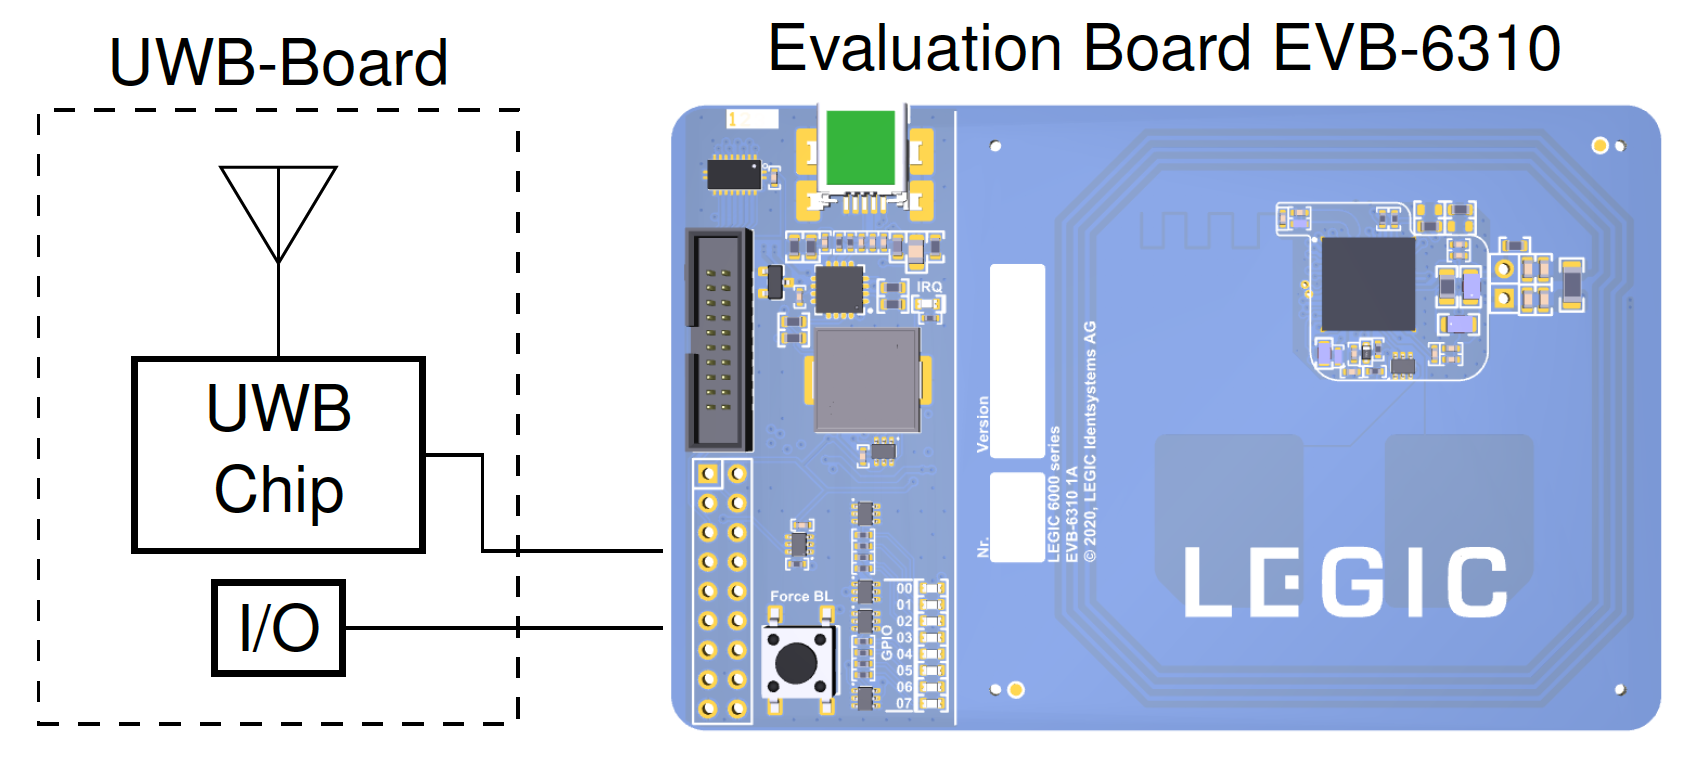
\includegraphics[width=11cm]{images/constellation_HW}
	\caption{Possible hardware arrangement}
	\vspace{-2ex}
	\caption*{\textbf{Source:} Original task definition}
	\label{fig:constellation_HW}
\end{figure}

To demonstrate general functionalities of UWB being
\begin{itemize}
	\item distance measuring between one or more UWB-Kits
	\item data communication between one or more UWB-Kits
	\item (optional) trilateration with three or more UWB-Kits
\end{itemize}

various use cases were defined in \cref{sec:use_cases}.

%With a designated hard- and firmware extension for the Legic Evaluation Board EVB-6310, testing of the new UWB-Technology should be made possible for LEGIC customers. The evaluation board is based on the LEGIC security chip SM-6310 which includes a customizable ARM CORTEX and supports Bluetooth Low Energy, NFC and RFID. %The UWB extension should preferably be realised with the silicon chip from the 3db Access AG and in the LRP-Mode.



%For the extension, UWB chips from 3db-Access should preferably be used. %, since they utilize the IEEE 802.15.4z standard.


%The existing Evaluation Board EVB-6310, based on the LEGIC security chip SM-6310, should be extended with UWB. This enables LEGIC customers to test the UWB-Technology. Today, the evaluation board implements 

	\newpage
\section{Product Requirements}
\subsection{Localization Methods}
%There are in general two ways the position of a tag in tow-dimensional space can be determined. 
There are several methods that can be used for localization with UWB. %localization methods can be used with UWB. 
The most common ones and the ones which were considered for this project are Two-Way Ranging (TWR), Time Difference of Arrival (TDoA) and Angle of Arrival (AoA). A minimum of three anchors are needed to localize one tag in two-dimensional space with TWR and TDoA. However, only one anchor is needed with AoA, but with multiple antennas. Furthermore, AoA is not supported by today's UWB chips, which leads to a more complex hardware, but it will likely be supported in the future. For these reasons, TWR and TDoA are going to be evaluated in this project. Additionally, it is assumed that the anchors have a known fixed position. %For this reason, TWR and TDoA are xof more interest and going to be evaluated in this project. 

\subsection{Technology}
Preferably, the UWB chips ATA83-50/-52 by 3db Access AG should be used, with which also the favourable LRP mode is available. As a substitute, the UWB chip DW1000 by Decawave can be used.

\subsection{Hardware}
For an UWB-Kit, the LEGIC evaluation board EVB-6310 and the additional UWB-Board are required. To demonstrate all the different use cases based on the localization methods above, at least four UWB-Kits (1 tag + 3 anchors) are needed and every UWB-Kit should contain the following input/output elements:
\begin{itemize}
		\item Buttons: for various user inputs (e.g. knob of key-fob)
		\item LEDs: output simulation (e.g. infected state, door lock status)
\end{itemize}

%The additional UWB-Board is powered by the LEGIC evaluation board. Also, for the design of the UWB-Board the UWB chip from %the 3db Access AG and the LRP UWB mode should preferably be used.

\subsection{Firmware}
For all use cases defined in \cref{sec:use_cases}, additional firmware for the LEGIC security chip SM-6310 is needed. A set of functions, which are used to configure the UWB chip and to perform the various communication and measurement tasks, should be implemented as modular as possible.
	\newpage
\section{Use Cases}
\label{sec:use_cases}
\subsection{UC1 Covid Tracker}
If a healthy person is within a defined range of an infected person for a defined time, the healthy person is notified and counted as an infected person from then onwards. To accomplish this, every person carries an UWB-Kit, which tracks his distance with TWR to other UWB-Kits and exchanges the infection state with them. 

\subsection{UC2 Hotel Door}
If a person comes close to a hotel door from the outside with the appropriate key, the door is unlocked and the person can enter the hotel room. As soon as the person with the key is inside the room, the door is locked again. The person can leave the room by mechanically unlocking the door. For every hotel room there is only one key containing one UWB-Kit, whereas the door-with-lock holds multiple UWB-Kits to determine the relative position of the key. This is accomplished with the use of TWR and TDoA. 

\subsection{UC3 (optional) Car Door}
If a person approaches a car with the appropriate car-key, the car only opens when the key comes from a defined direction. Therefore, the car-key consists of one UWB-Kit, while the car comprises multiple UWB-Kits. This allows the car to determine the relative position of the car-key using TDoA.
	%\section{Global Requirements}

% % % % % % % % % % % % % % % % % % % % % % % % % % % % % % % %
% ANHANG
% % % % % % % % % % % % % % % % % % % % % % % % % % % % % % % %
\appendix


%Nummerierung wieder auf roemisch umschalten

%\newpage
%\section{References}
%\label{anx:ref}
%% Do not repeat items covered in other documents or in a global project definitions and acronyms document
%\renewcommand{\refname}{} %kein Titel vor Literaturverzeichnis
%\vspace{-1.2cm}
%\bibliographystyle{ieeetr} %Literatur durchnumerieren
%\bibliography{lit}
%\nocite{*} %Alle Literatur aufführen
	
\end{document}